% Alternative Options:
%	Paper Size: a4paper / a5paper / b5paper / letterpaper / legalpaper / executivepaper
% Duplex: oneside / twoside
% Base Font Size: 10pt / 11pt / 12pt
\documentclass[a4paper, twoside, 11pt]{report}


% This file contains all the packages used in the template
% Remove or add new packages to suit your needs




%% Language %%%%%%%%%%%%%%%%%%%%%%%%%%%%%%%%%%%%%%%%%%%%%%%%%

% Bytt til norsk for å få norsk innholdsfortegnelse
\usepackage[USenglish]{babel} % norsk, francais, polish, spanish, ...

\usepackage[utf8]{inputenc}
\usepackage[T1]{fontenc}

%% Andre pakker %%%%%%%%%%%%%%%%%%%%%%%%%%%%%%%%%%%%%%%%%%%%%%%%%
\usepackage{hyperref}
\usepackage{biblatex}
\usepackage{csquotes}
\usepackage{graphicx} %%For loading graphic files
\usepackage{amsmath}
\usepackage{amsthm}
\usepackage{amsfonts}
\usepackage{eso-pic}
\usepackage{transparent}
\usepackage{float} %% For using H flowt specifier
\usepackage{svg}
\usepackage{xcolor} %% for color text
\newcommand{\node}[1]{\textcolor{blue}{#1}}
\newcommand{\topic}[1]{\textcolor{red}{#1}}
\usepackage{listings}



%\usepackage{auto-pst-pdf} % Enables the psfrag tool
%\usepackage{psfrag}% Enables the psfrag tool
\usepackage{psfrag}
\usepackage{authblk}


%% For programming text input %%%%%%%%%%%%%%%%%%%%%%%%%%%%%%%%%%%%%%%%%%%%%%%%%

\usepackage[framed,numbered,autolinebreaks,useliterate]{mcode}
\usepackage{listingsutf8}
% Small fix for special characters
\lstset{literate=
  {á}{{\'a}}1 {é}{{\'e}}1 {í}{{\'i}}1 {ó}{{\'o}}1 {ú}{{\'u}}1
  {Á}{{\'A}}1 {É}{{\'E}}1 {Í}{{\'I}}1 {Ó}{{\'O}}1 {Ú}{{\'U}}1
  {à}{{\`a}}1 {è}{{\`e}}1 {ì}{{\`i}}1 {ò}{{\`o}}1 {ù}{{\`u}}1
  {À}{{\`A}}1 {È}{{\'E}}1 {Ì}{{\`I}}1 {Ò}{{\`O}}1 {Ù}{{\`U}}1
  {ä}{{\"a}}1 {ë}{{\"e}}1 {ï}{{\"i}}1 {ö}{{\"o}}1 {ü}{{\"u}}1
  {Ä}{{\"A}}1 {Ë}{{\"E}}1 {Ï}{{\"I}}1 {Ö}{{\"O}}1 {Ü}{{\"U}}1
  {â}{{\^a}}1 {ê}{{\^e}}1 {î}{{\^i}}1 {ô}{{\^o}}1 {û}{{\^u}}1
  {Â}{{\^A}}1 {Ê}{{\^E}}1 {Î}{{\^I}}1 {Ô}{{\^O}}1 {Û}{{\^U}}1
  {Ã}{{\~A}}1 {ã}{{\~a}}1 {Õ}{{\~O}}1 {õ}{{\~o}}1
  {œ}{{\oe}}1 {Œ}{{\OE}}1 {æ}{{\ae}}1 {Æ}{{\AE}}1 {ß}{{\ss}}1
  {ű}{{\H{u}}}1 {Ű}{{\H{U}}}1 {ő}{{\H{o}}}1 {Ő}{{\H{O}}}1
  {ç}{{\c c}}1 {Ç}{{\c C}}1 {ø}{{\o}}1 {å}{{\r a}}1 {Å}{{\r A}}1
  {€}{{\euro}}1 {£}{{\pounds}}1 {«}{{\guillemotleft}}1
  {»}{{\guillemotright}}1 {ñ}{{\~n}}1 {Ñ}{{\~N}}1 {¿}{{?`}}1
}


%% Line Spacing %%%%%%%%%%%%%%%%%%%%%%%%%%%%%%%%%%%%%%%%%%%%%
%\usepackage{setspace}
%\singlespacing        %% 1-spacing (default)
%\onehalfspacing       %% 1,5-spacing
%\doublespacing        %% 2-spacing


%% Other Packages %%%%%%%%%%%%%%%%%%%%%%%%%%%%%%%%%%%%%%%%%%%
%\usepackage{a4wide} %%Smaller margins = more text per page.
\usepackage{fancyhdr} %%Fancy headings
%\usepackage{longtable} %%For tables, that exceed one page

\usepackage{color}
\definecolor{darkgreen}{rgb}{0.3,0.6,0.3}

\parindent 0mm
\setlength{\oddsidemargin}{0mm}
\setlength{\evensidemargin}{0mm}
\setlength{\topmargin}{-20mm}
\setlength{\textwidth}{165mm}
\setlength{\textheight}{260mm}

\hypersetup{
   pdfauthor={UiA Mechatronics Student},
   pdftitle={Technical Report},
   pdfkeywords={report, mechatronics, University of Agder},
   pdfsubject={Project Report},
   colorlinks=true,
   citecolor=darkgreen,
   urlcolor=darkgreen,
   linkcolor=black,
   pdfstartview=Fit,
   pdfpagelayout=SinglePage,
   pdfcreator=pdflatex,
   pdfproducer=pdflatex
}


\addbibresource{bibliography.bib}

\begin{document}
%\rmfamily




\pagestyle{empty} %No headings for the first pages.


\begin{titlepage}


%%%% Select the correct front page by changing the reference below %%%% 

% Figures/Frontpage/forside_bachelor_eng.pdf
% Figures/Frontpage/forside_bachelor_nor.pdf
% Figures/Frontpage/forside_master_eng.pdf
% Figures/Frontpage/forside_master_nor.pdf

\AddToShipoutPicture*{
    \put(-4,0){
        \parbox[b][\paperheight]{\paperwidth}{%
            \vfill
            \centering
            % Change the reference in this line to change front page
            % forside_bachelor_eng.pdf, forside_bachelor_nor.pdf 
            % forside_master_eng.pdf, forside_master_nor.pdf
            
\includegraphics[width=1.275\textwidth]{Figures/Frontpage/forside_master_eng.pdf}%
            \vfill
        }
    }
    \put(0,0){%
        \transparent{0}\textcolor{white}{\rule{\paperwidth}{\paperheight}}
    }
}

%%%% Type in your data here %%%% 

\newcommand{\projectTitle}{Autonomous platooning}
\newcommand{\projectSubTitlel}{}
\newcommand{\authors}{LARS MUGGERUD}
\newcommand{\supervisor}{Ajit Jha}

\newcommand{\projectYear}{2023}
\newcommand{\facultyName}{Faculty of Engineering and Science}
\newcommand{\departmentName}{Department of Engineering and Sciences}




%%%% Page Layout %%%% 
\begin{tabular}{p{12cm}}
                                            \\[5cm]
    \LARGE{\textsc{\textbf{\projectTitle}}} \\[1.5cm]
    \projectSubTitlel                       \\[2.5cm]
    \large{\authors}                        \\[9cm]
    \Large{SUPERVISOR}                      \\
    \supervisor
\end{tabular}



\vfill


\textbf{University of Agder, \projectYear} \\
\small{\facultyName \\
\departmentName}
\vspace{1cm}
\end{titlepage}

  
\clearpage

\pagenumbering{gobble}
\pagenumbering{roman}


\newpage

\chapter*{Declaration}



\chapter*{Acknowledgements}
I want to thank my supervisor Ajit Jha for his knowledge and support during this thesis. I want to thank Didrik Robserud and Ørjan Øvsthus my fellow student also working with the Husky UGV for accordance and support. Lastly i want to thank my family and my girlfriend for their support.  
\addcontentsline{toc}{chapter}{Acknowledgements}

\clearpage
\chapter*{Abstract}
\addcontentsline{toc}{chapter}{Abstract}

\clearpage

\tableofcontents
\cleardoublepage %The first chapter should start on an odd page.
\pagestyle{plain} %Now display headings: headings / fancy / ...

%List of Figures
\listoffigures
\addcontentsline{toc}{chapter}{List of Figures}
\clearpage
\textcolor{white}{.}
\thispagestyle{empty}
\newpage

%List of Tables
\listoftables
\addcontentsline{toc}{chapter}{List of Tables}
\clearpage

\textcolor{white}{.}
\thispagestyle{empty}
\newpage

\clearpage
\pagenumbering{arabic}





\chapter{Introduction}
This template is meant as an example
of how a technical report can be
structured. Discuss the table of content and the names of the chapters with the
group members and supervisor to suit your specific report.\\

\section{Some \LaTeX{} Examples}

\subsection{Using the Bibliography}

This is an example of how to use the bibliography and citations. Cite to Einstein \cite{einstein}, or something else \cite{dirac}.\\


\subsection{Writing Mathematics}

This is some examples of how to write math in \LaTeX.

\begin{equation}
    y(x) = \frac{\sin x}{e^x}
    \label{eq:label1}
\end{equation}

We can refer to the equation by using the label, like this: eq \ref{eq:label1}.\\

We can choose whether to number the equation or not:
\begin{equation*}
    y(x) = \frac{\sin x}{e^x}
\end{equation*}

Lastly, we can write inline math: $y = a \cdot x + b$ 

\subsection{Programming Code}

Inline MATLAB code: \mcode{variabel = max(input)}\\

MATLAB code in section:
\begin{lstlisting}
for i = 1 : 10
% Skriv kode her
end
\end{lstlisting}


\newpage

\subsection{Inserting Tables}

\begin{table}[h]
    \centering
    \begin{tabular}{c|c}
        Variable    &   Value   \\
        \hline
         $\theta$   &   10      \\
         $\omega$   &   40 
    \end{tabular}
    \caption{The table Caption}
    \label{tab:label1}
\end{table}

This table can be referred to by using the label, like this: table \ref{tab:label1}.


\subsection{Including figures}

\begin{figure}[h]
    \centering
    
\includegraphics[width = 0.7\textwidth]{Figures/Frontpage/forside_master_nor.pdf}
    \caption{The figure Caption}
    \label{fig:label1}
\end{figure}

This figure can be referred to by using the label, like this: figure \ref{fig:label1}.


\subsection{Multicolumn}

\begin{minipage}{0.45\textwidth}

    \vspace{-4cm}
    Text to describe for example a photo. Here we can write really long sentences just to prove the concept of the minipage, which is that the text will follow the width of the minipage that we have specified. In this case it was 45 \% of the total textwidth, with a small spacing in between, using the command "hspace". If we would like the text to start further up in the minipace, we can use the command "vspace" in front of the text, to shift it vertically.

\end{minipage}
\hspace{0.05\textwidth}
\begin{minipage}{0.45\textwidth}
 
    
\includegraphics[width = \textwidth]{Figures/Frontpage/forside_bachelor_nor.pdf}

\end{minipage}





\chapter{Theory}
% every  chapter has intro and conclution 
%aj a paragraph explaining what is mentioned in the chapter. write about the building blocks of yuour thesis. please see the teams where i have outlined them. then each section becomes the theory or working principle of the individual components.
In this chapter i will present the concepts and theory used in autonomous platooning.  
\section{Robotics}
Robotics is a vast and interdisciplinary field that involves the design, construction, operation, and use of robots. From manufacturing and transportation to healthcare and entertainment, robots are used in a wide range of industries and applications to automate tasks, enhance human capabilities, and explore new frontiers.
In this particular project, the focus is on autonomous driving robots. To achieve autonomous driving in this project the robots used motion estimate(odometry), vision(LiDAR) and software(ROS2 and Nav2). 
%aj remove

\subsection{Autonomous platooning}
Autonomous platooning is a technique used in transportation, where a group of vehicles travel closely together in a formation, with one vehicle leading the group and the others following. The leading vehicle is typically driven by a human driver or an autonomous system, and the following vehicles are autonomous and communicate with the leading vehicle to maintain the desired distance and speed. The purpose of autonomous platooning is to increase efficiency and safety on the roads. By traveling in a close formation, the vehicles can reduce their air resistance and save fuel. Additionally, the autonomous systems can react more quickly to changes in the road conditions, such as traffic congestion or accidents, reducing the risk of collisions and improving overall safety. Autonomous platooning is a part of robotics.
%aj remove from here and may be put it in introduction

%background /theory should be about - autonomous navigation, slam, collision avoidance, networked communication ... see teams
\subsection{Odometry}
Odometry is the use of data from sensors on a mobile robot to estimate its motion, specifically its position and orientation changes over time. In robotics wheel encoders and Inertial Measurement Units (IMUs) are used as sensors. Estimates from wheel encoders struggles with various sources of error, such as slippage, uneven terrain and imperfect sensors. These errors can accumulate over time and result in significant deviations from the actual position and orientation of the robot[]. 
IMUs are sensors that measure the linear and rotational motion of a robot by sensing changes in acceleration and angular velocity. Although IMUs are useful for providing real-time data on a robot's motion, they are also subject to various sources of error that can affect their accuracy, such as bias, noise, drift, and temperature changes. 
To solve the problems with wheel encoders and IMUs, a common approach is to use sensor fusion techniques, which combine data from multiple sensors to obtain a more accurate estimate of the robot's position and orientation. One common method for sensor fusion is the Extended Kalman Filter (EKF). 

\subsection{EKF filter}
The EKF (Extended Kalman Filter) is a type of recursive Bayesian filter commonly used in robotics and control systems for estimating the state of a system with noisy sensor measurements. The EKF is an extension of the Kalman Filter that is designed to handle nonlinear systems by using a linear approximation of the system's dynamics and measurement functions around the current state estimate. The EKF estimates the system state by recursively updating a predicted state estimate using a model of the system's dynamics and the measurements received from sensors. The EKF also estimates the uncertainty of the state estimate using a covariance matrix, which is updated at each time step based on the predicted and measured uncertainties. The EKF is widely used in robotics applications, such as localization and mapping, where it can estimate the position and orientation of a robot based on noisy sensor data, such as GPS, IMU, or visual odometry.
%aj these two above sections can be in navigation

%hardware section remove here put in methodology /experimental setup
\section{Hardware}

The hardware used in this thesis is presented in Table \ref{tab:HW_list}.

\begin{table}[H]
    \centering
    \begin{tabular}{c|c|c}
        Name                    & Reference name    & Short description  \\ \hline
        Clearpant Husky         & Husky             & Medium sized wheeled robot \\
        Nvidia Xavier 1         & Xavier1           & Compact computer controlling the Husky\\
        Ouster OS-1-64          & OS1               & 3D LiDAR on the Husky \\
        UM7 Orientation Sensor  & UM7               & Inertial measurement unit(IMU)  \\
        Husky's wheel encoder   & Wheel encoder     & Measures the movement of the wheels\\
        TurtleBot3              & TB3               & Small sized wheeled robot   \\
        Nvidia Xavier 2         & tb                & Compact computer Controlling TB3  \\
        LDS-01                  & LDS-01            & 2D LiDAR on TB3 \\
        OpenCR 1.0              & OpenCR 1.0        & Microcontroller with IMU for robotics \\
        
    \end{tabular}
    \caption{List of hardware}
    \label{tab:HW_list}
\end{table}

\subsection{Xavier}
Xavier or NVIDIA Jetson AGX Xavier Developer Kit \cite{xavierguide} is an compact computer for AI applications. With the size 105mm x 105mm x 65mm and the power source being 9 - 20 volts its practical for mobile robots. 

The Nividia computers come with their own Linux version called JetPack, based on Ubuntu. The JetPack system includes AI applications. JetPack and the GPU is the reason why the Xavier is suitable for AI applications. The CPU of the Xavier has an ARM architecture. A WiFi module can be attached and is in this project.

\subsection{Sensors}

\paragraph{LiDAR}(Laser imaging, Detection, and Ranging) is a method of measuring distances with laser. The principle is sending a laser beam at a target, sensing the reflection and calculating the distance based on time between laser sent and received. 

TurtleBot3 uses a LiDAR called LDS-01 and the Husky uses Ouster OS-1-64. Table \ref{tab:lidar_data} provides relevant data for the LiDAR's. 

\begin{table}[h]
    \centering
    \begin{tabular}{c|c|c}
        Specifications          & TrutleBot3        & Husky             \\ 
                                & LDS-01            & Ouster OS-1-64    \\ \hline
        Range                   & 120 - 3,500mm     & 0.8m - 120m       \\ \hline
        Vertical resolution     & 1 channel         & 64 channel        \\ \hline
        Angular Range           & $360^\circ$       & $360^\circ$       \\ \hline  
        Power source            & Micro USB         & Barrel jack       \\  
                                & 5 volts           & 24 volts          \\ \hline
        Data line               & Micro USB         & Ethernet          \\       
    \end{tabular}
    \caption{LiDAR data for LDS-01\cite{lds01} and OS1 \cite{OS1Datasheet}}
    \label{tab:lidar_data}
\end{table}

\paragraph{Inertial Measurement Unit (IMU)} is an electronic device that uses accelerometers, gyroscopes, and sometimes magnetometers to measure and report a body's specific force, angular rate, and occasionally its orientation.

\paragraph{Rotary encoders} are electro-mechanical devices that convert the angular position or rotation of a shaft into an electrical signal. They are commonly used in robotics, automation, and other control systems to measure the position and speed of rotating objects, such as wheels, motors, and joints. Rotary encoders typically consist of a rotating disk or shaft with evenly spaced markers or slots, and a stationary sensor or detector that reads the changes in the markers or slots as the shaft rotates. There are two main types of rotary encoders: incremental and absolute. Incremental encoders provide relative position and speed information, while absolute encoders provide absolute position information. Rotary encoders can be connected to a microcontroller or other processing unit to read and interpret the electrical signal, and use it to control the movement and position of a robot or other device.

\subsection{Husky}
The Husky UGV \cite{huskyugv} is an medium sized UGV(unmanned ground veichle) from Clearpath. It have fire wheels and a footprint of 990mm x 670mm. It is powered by two 24volts battery's in series, total 48 volts. There is three power outputs for external components 5V, 12V and 24V fused at 5A each. A motor drive and wheel where included, the mini-ITX and IMU where not. 

The front and back wheel of each side is mechanical connected, and power by one motor. Therefor in able to turn the Huksy will scid, this makes the turning and odometry prediction form the wheel encoders inaccurate. 
(This makes the odometry more dependent on the IMU and should be in mind when tuning the ekf filter or similar data fusing methods.) 

The size and sciding of the Huksy combined with the range of the LiDAR can be an issue when driving autonomous with Nav2 inside. It acts clumsy with the turning blind zone under 80cm. 

\subsection{TurtleBot3}
The TurtleBot3(Waffle Pi) is small robot provided by Open Robotics and ROBOTIS \cite{turtlebot3}. The footprint of the robot is 138mm x 178mm, its driven by two front wheels and have two ball casters in the back. Therefor the TurtleBot3 has differential drive, witch is a precise way to turn[]. 

\paragraph{OpenCR1.0} is a multi purpose board on the TurtleBot3\cite{opencr10}. This board connects the battery, and powers the Xavier and motors for the wheels. The control signal for the wheels comes from the Xavier through the OpenCR1.0 int the wheels. 
A LiDAR is included as well as an IMU on OpenCR1.0 board.


%aj whole software section needs to be removed.
\section{Software}

\subsection{Ubuntu}

Ubuntu is an open source operating system(OS) based on Linux\cite{ubuntu}\cite{osi}. It the most popular Linux distribution and the main OS for ROS2. ROS2 can be used on Windows and Mac as well but is sub optimal. Ubuntu have two main forms desktop and server. Desktop provides a graphical user interface(GUI). Ubuntu server dose not have a GUI, it is just a text-based user interfaces(TUI). The server is more demands less possessing power and storage. 


\paragraph{SSH} or Secure Shell is a network protocol for communication between two computers witch is encrypted. The two computers have to be on the same network. SSH is a terminal based program, therefor there is no GUI just a TUI. 

In robotics SSH is commonly used. Often its not practical or possible to connect the robots computer to keyboard and a monitor. A lot of robots have computers running a TUI based OS, so a monitor wound not provide more information than SSH. 

\subsection{ROS2} or robot operating system 2 \cite{rosfoxydocs} is a meta OS installed on top of an other OS. The OS most commonly used is Ubuntu. ROS2 can be described as a base for building robot applications with a set of software libraries and tools. ROS2 is open source and has a large community, this is essential. The large community means that a its a lot of help online. Open source makes is easier to make ROS2 software to different hardware. 

\subsubsection{ROS2 components} 

A large part of ROS2 is communication with the messages. Messages refers to data this can be single variables like "int", "float", "string" and so on. Bigger data types like "Twist.msg" and "Odometry.msg" is also messages, this often contain hierarchy of data. 
Table \ref{tab:ROS2_topics} shows list of common ROS/ROS2 topics.
\begin{table}[H]
    \centering
    \begin{tabular}{c|c}
       Topic name       & Function          \\ \hline
        /cmd\_vel       & Velocity command  \\
        /odom           & Odometer          \\
        /scan           & 2D laser scan     \\
        /points         & 3D laser scan     \\        
        /imu/data       & IMU data          \\
    \end{tabular}
    \caption{Caption}
    \label{tab:ROS2_topics}
\end{table}

The standard topic names are convenient but can cause problems when there is multiple types of the same sensor. Namespace solves this problem by putting "/namespace" in front of \topic{/generic\_topic\_name}.  

\paragraph{Nodes} in ROS2 is a lightweight and modular process that performs a specific computation. Each node is identified by a unique name within the ROS2 system. 
ROS2 nodes can be described by what they are commonly used for. 

\begin{itemize}
    \item Publish sensor data: A ROS node can read data from sensors, such as cameras or lidars, and publish it to a ROS topic for other nodes to consume like \topic{/scan} and \topic{/points}.
    
    \item Control a robot: A ROS node can send commands to a robot's motors or actuators to control its movement or behavior based on topics like \topic{/cmd\_vel}.
    
    \item Process data: A ROS node can receive data from other nodes and perform calculations or transformations on it, such as filtering or mapping for example a EKF filter node.
    
    \item Provide a user interface: A ROS node can provide a graphical user interface (GUI) or command-line interface (CLI) for users to interact with the system like teleop or Rviz.
    
    \item Manage communication: A ROS node can act as a bridge between different communication protocols or systems, allowing them to exchange data using ROS messages.
    
\end{itemize}

Nodes communicate with each other by publishing messages to topics or subscribing to topics to receive messages. Nodes can also communicate with each other using services, which provide a request/response communication pattern. ROS2 nodes can also communicate with each other using actions, which provide a more complex form of request/response communication pattern that involves feedback and cancellation. Nodes can be started up directly for the terminal or a launch file. 

\paragraph{Launch files} is needed in bigger ROS2 project where there is often a lot of different hardware that needs to be stated or launched to start a complete robot. Python or xml launch files is a script for launching multiple nodes and send arguments into them. Launch files can also launch other launch files, convenient because this is often provided with complete robots. 

\paragraph{ROS arguments} can be passed into nodes and launch files, and alter the way they work. What type of arguments is available depends on the function of the node or launch file. Arguments can be passed directly into nodes in the terminal like this : 
\begin{lstlisting}[language=bash]
  ros2 run demo_nodes_cpp talker --ros-args -r __ns:=/namespace
\end{lstlisting}
Nodes can also resive arguments in a launch file like this: 
\lstinputlisting[language=Python]{code/talker_launch.py}

For launch files argument function the same way just a bit different syntax. To check if arguments can be bassed into a launch file write --show-args at the end of the launch command, for example: 
\begin{lstlisting}[language=bash]
  ros2 launch turtlebot3_bringup robot.launch.py --show-args
\end{lstlisting}

\paragraph{Parameter files} is a .yaml file with multiple arguments or configurations. Often parameter files can be passed in as an argument.

\paragraph{ROS2 packages} is a standard way to structure ROS2 code, making it essay integrate custom code into ROS2 and share it. A typical ROS2 package contains nodes, launch files and parameter files. 

\paragraph{rqt} is a visualisation tool for ROS2. It provides a map of nodes and topics on the local network. This is a great tool for debugging. 

\paragraph{Gazebo} is a physics-based simulator for testing and developing robotics algorithms. It uses models to represent robots and objects in the simulated environment. Gazebo supports a plugin system for extending its functionality. It provides a GUI for visualizing and interacting with the simulation, witch also works great with Rviz.

\paragraph{Rviz} is a 3D visualization tool for ROS that allows users to view and interact with robot data in real-time. It can display data such as point clouds, laser scans, and 3D models of robots and their environments. Rviz allows users to change the perspective of the visualization and interact with the data using mouse and keyboard commands. It can also be used to configure sensors and other components of a robot system by visualizing their data and properties. In summary, Rviz is a powerful 3D visualization tool for ROS that allows users to interact with robot data in real-time and visualize sensor data and properties.

\paragraph{teleop_twist_keyboard} or just teleop is a build in tool in ROS2 for controlling robots from the keyboard. It dose this by publishing velocity control from keyboard input on the "/cmd\_vel" topic.   

\paragraph{Nav2} (Navigation Stack 2) \cite{rosnavigation} is a high-level open-source software framework for autonomous robot navigation in ROS2. It provides a set of reusable and configurable software components for creating complex navigation behaviors for mobile robots, including path planning, localization, obstacle avoidance, and control. Nav2 is built on top of the ROS2 middleware and leverages other ROS2 packages for communication and hardware abstraction. It also provides interfaces for integrating with other navigation systems and tools, such as Gazebo and RViz. Nav2 is designed to be modular and extensible, allowing developers to customize and add new navigation behaviors to meet the specific requirements of their robots and environments.

Nav2 API(application programming interface)\cite{rosnavAPI} is a set of commands for interacting with Nav2 from Python. Examples of commands can be send a goal, receive position and check if a task (rout) is complete.    


\chapter{Methods in ...} %aj material and method

%aj 3.1 experiment setup
%3.2 methodology
%3.2.1  autonomous navigation of husky
%3.2.2 autonomous navigation of tb
%3.2.3 mimic algorithm
%3.2.4 platooning

%aj first para(s) should be without section where you explain what is in the chapter. write about the  algorithm (a) imitation/mimic and (b) paltooning
\section{Introduction of method}
In this chapter the setup of Husky and TB3 both hardware and software will be explained. Then how both where setup to drive autonomous independently. Lastly the platooning algorithms will be explained. 

%aj remove. good for handover
Before getting into the setup of Husky and TB3 it is necessary to explain the the custom packages made for this project $masteruia$ \cite{masteruia} and $uia\_husky\_0776$ \cite{uiahusky}. 

There where three project on the Husky at the same time, so a common GitHub was made $uia\_husky\_0776$. All the software used by the Husky in this project is launched from the $uia\_husky\_0776$ such as packages for Husky, OS1, UM7 and "pointcloud\_to\_laserscan".

$masteruia$ is the other GitHub used in the project and contains two packages $uia\_husky\_0776$ and $tb3\_cpp$.
First off the folder called $uia\_husky\_0776$ is a copy of the one talked about above. The folder was made when trying to launch the Husky with namespace, this task was not completed. 
The $tb3\_cpp$ is standard ROS2 CMake package consisting a launch file for TB3, nodes for Nav2 API and platooning algorithm. 
                      
%aj suggest to follow the above structure. the content aslo has to be rewritten. mention about UGV, sensors - lidar, IMU, computing platform - xavier 1 .
\section{Husky}
\subsection{Hardware}
This section will describe the setup of the Husky and its components. 

The IMU was glued to the center of the tray, connected with a USB to the Xavier. 
In the Husky there are two Xavier only one of them is used in this project. The one used is Xavier1 the other is Xavier2. Both of the Xaviers where placed in the tray and secured with a 3D printed mount. The Xaviers where lacking USB ports so both of them got a USB hub. 
The Ouster LiDAR has two components the laser scanner and the power/data brick. The scanner is mounted on top of a aluminum frame in the front for long distance scanning. The brick is blued to the front wall off the tray, connected to 24 volt barrel jack and Ethernet form the router. 
The router is mounted in the front of the aluminum frame powered by 12 volt barrel jack. Xavier and Xavier2 is connected with Ethernet, Xavier also has a WiFi connection. 
\begin{figure}[H]
  \centering
  \begin{minipage}[b]{0.4\textwidth}
    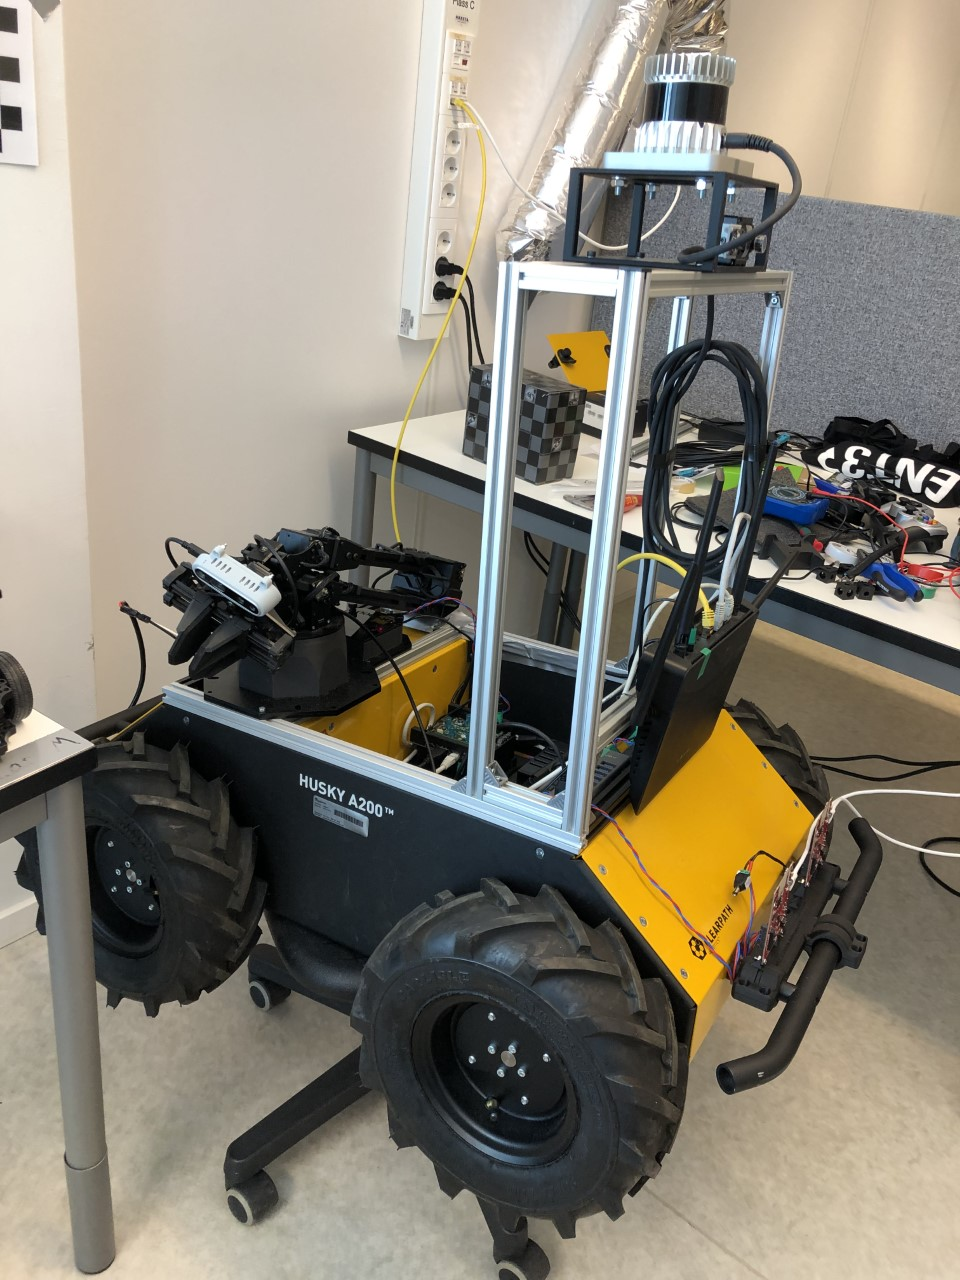
\includegraphics[width=\textwidth]{Figures/images/husky_irl.jpg}
    \caption{Photo of Husky}
    \label{fig:husky_irl}
  \end{minipage}
  \hfill
  \begin{minipage}[b]{0.59\textwidth}
    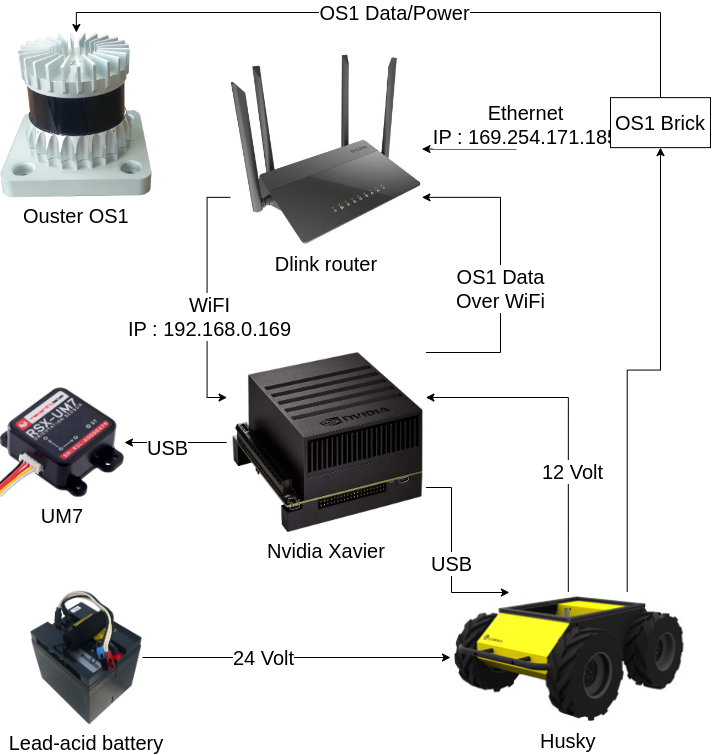
\includegraphics[width=\textwidth]{Figures/drawio/Husky_HW.drawio.png}
    \caption{Husky hardware map, this dose not include components on the Husky used in other projects}
    \label{fig:Husky_HW}
  \end{minipage}
\end{figure}
%aj font size needs to be increased, its not redable
\subsection{Software}
This section will describe thee setup of the Husky without Nav2, the 
%aj the section describes (not will describe)
"base" setup of the Husky. For less comfusion all \topic{topics} and \node{nodes} have colors and there ROS2 name. 
The Xavier1 on the Husky is runnning Ubuntu 20.04 Desktop
%since you use only one xavier call it xavier
\cite{ubuntu20_04} with ROS2 foxy \cite{rosfoxyinstall} and galactic \cite{rosgalacticinstall}, Nav2 binary \cite{rosnavinstall}, Husky foxy Debian packages \cite{huskyinstall} and $uia\_husky\_0776$ \cite{uiahusky}. When setting up the ROS2 software Rviz and rqt was used to test all components. \newline
    
$uia\_husky\_0776$ launches packages for Husky, OS1, UM7 and $pointcloud\_to\_laserscan$. A launch file was made to launch it all at once "husky.launch.py" in "uia\_husky\_0776/husky\_group/launch/".


Clearpath provides binary packages for the Husky in ROS2 foxy, because of this the hole project was set up foxy in the beginning . The Clearpath packages provides the essential software for making the husky move with ROS2.

%aj why write about another project?
An other project on the Husky was pick and place and used the ViperX 300 Robot Arm. This arm was better to set up with Galactic, so the project was converted to Galactic. Foxy and Galactic are similar and didn't cause any issues, except for with the Husky package. Clearpath did not provide binary packages for the Husky in Galactic just source. This source files did not initially work on the Husky. The student working on pick and place made some changes to the source files, making them work. Still the source files on Galactic are more unstable then Foxy. Therefor "base\_launch.py" is launched in Foxy and the rest of the project in Galactic. 

%aj need to understand what you have used
The Husky is launched with the $husky.launch.py$ from $husky\_group$ in the $uia\_husky\_0776$. $husky.launch.py$ pass in parameters and starts $base\_launch.py$, \node{um7\_node}, $os1_launch.py$ and \node{pointcloud\_to\_laserscan}. 

$base\_launch.py$ starts up the /joy\_teleop and /robot\_state system and the nodes \node{/twist\_mux}, \node{/huksy\_velocity\_controller} and \node{/ekf\_node}. 

\begin{itemize}
    \item joy\_teleop system converts a Logitech joystick controllers signal into \topic{joy\_teleop/cmd\_vel} a standard velocity massage with namespace. 
    
    \item \node{/twist\_mux} converts \topic{/cmd\_vel} with and without namespaces to \topic{/husky\_velocity\_controller/cmd\_vel\_unstamped} and sends it into \node{/huksy\_velocity\_controller}. Every velocity command for the Husky goes though the \node{/twist\_mux}, joystick, keyboard and Nav2. 
    
    \item \node{/huksy\_velocity\_controller} controlles the motors and publishes \topic{/odom} based on the wheel encounters on the Husky. 
    
    \item \node{/ekf\_node} fuses odometry(\topic{/odom}) and IMU(\topic{/imu/data}) to \topic{"/odometry/filtered"} to localize the Husky with greater precision[need a cite?]. 
    
    \item The /robot\_state system combines the URDF with the joint state of the wheels to create a accurate model of the Husky in Rviz. 
    
\end{itemize}

The UM7 ROS2 package where found on GitHub \cite{um7imu}. This packages launches a node called \node{/um7\_dirver} publishing data from the IMU on topic \topic{/imu/data}, into \node{/ekf\_node}.
\\ \newline
Ouster has a well documented GitHub \cite{ousterros} with ROS2 drivers for there hardware, including the OS1. The package starts up a node called \node{/ouster\_driver} witch publishes \topic{/points}. 
Since Nav2 uses \topic{/scan} as perception topic, a packages called "pointcloud\_to\_laserscan" \cite{pcl2laser} was installed to make the OS1 communicate with Nav2. "pointcloud\_to\_laserscan" was also found on GitHub . 

This image represents software of the Husky in a rqt format where 
ovals are \node{nodes} and squares is \topic{topics}. This dose not include Nav2. The original rqt image can be found here \ref{Appendix:HuskySWmap}. 

% this should be at the beginning and then eplain this figure in detail
\begin{figure}[H]
    \centering
    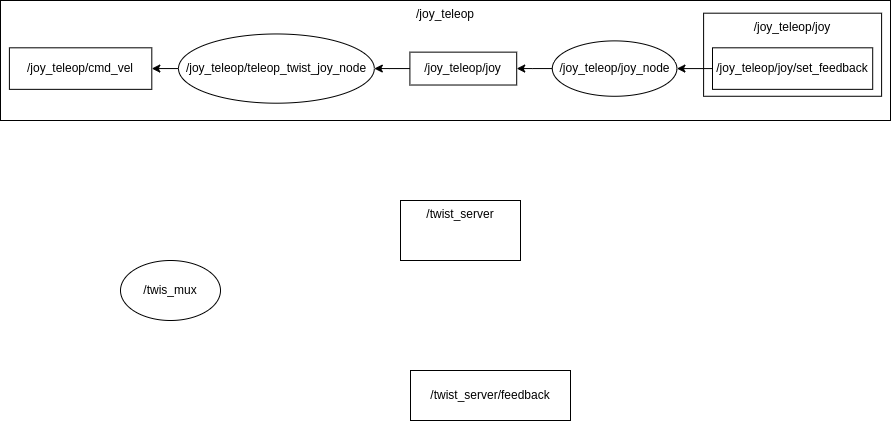
\includegraphics[width = 1\textwidth]{Figures/drawio/husky_rqt.drawio.png}
    \caption{Husky software map}
    \label{fig:HuskySW}
\end{figure}
% images neeed to be refrenced 

%aj use simple present. also write what you have done. All the failed attempt goes to discussion
\section{TurtleBot3}
\subsection{Hardware}
The TurtleBot3 started with no battery and was driven by a Raspberry Pi. The Pi was running Ubuntu Server and had an old student project saved. It had performance issues, writing in the TUI was choppy. The Pi was flashed with Ubuntu Server 20.04 in an attempt to increase the performance. This did not work, and therefor it was decided tho switch out the Pi. A Xavier was available, it is same as the Husky is using and was therefor chosen. The TurtleBot3 uses a battery similar to RC Cars, RC battery's was ordered though a local hobby store. Figure \ref{fig:TB3HW} shows the map of the TB3 hardware. 

\begin{figure}[H]
  \centering
  \begin{minipage}[b]{0.4\textwidth}
    \includegraphics[width=\textwidth]{Figures/images/TB3_irl.png}
    \caption{Photo of TB3}
    \label{fig:TB3_irl}
  \end{minipage}
  \hfill
  \begin{minipage}[b]{0.59\textwidth}
    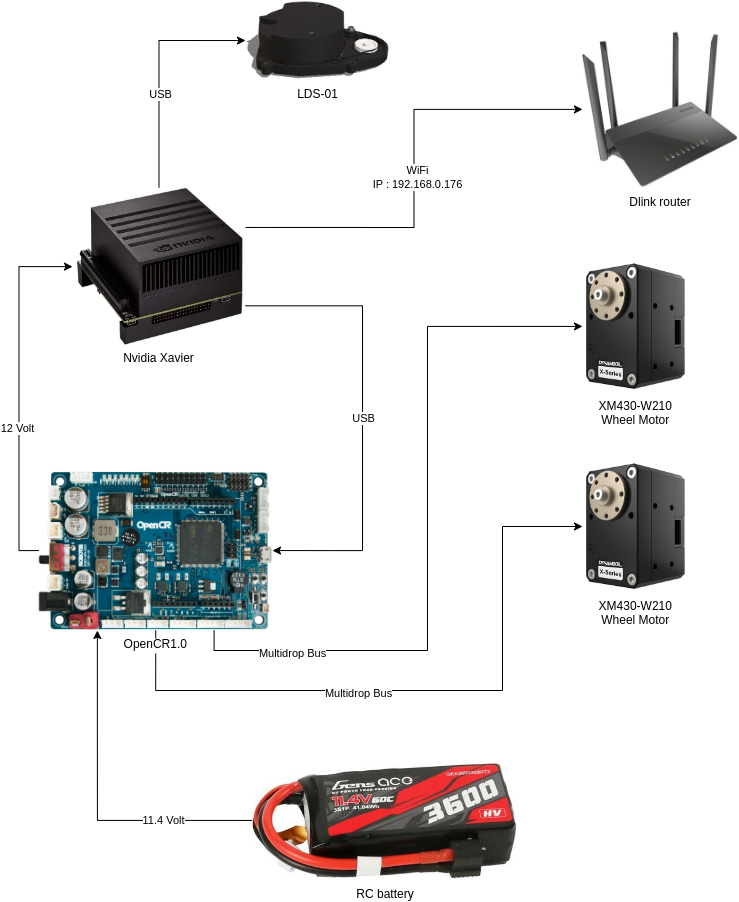
\includegraphics[width=\textwidth]{Figures/drawio/TB3_HW.drawio.png}
    \caption{TurtleBot3 hardware map}
    \label{fig:TB3HW}
  \end{minipage}
\end{figure}


%aj need to discuss to understand better. I guess fig 3.6 and 3.7 should be demonstrated first and explain them.
\subsection{Software}

This will describe the setup of the TB3 without Nav2, the "base" setup TB3.  
The name of user on the TB3 Xavier is tb and will be the reference. tb is running Ubuntu 20.04 Desktop \cite{ubuntu20_04} with ROS2 galactic Debian(binary) \cite{rosgalacticinstall}, TB3 packages binary \cite{turtlebot3galactic}, Nav2 binary \cite{rosnavinstall} and $masteruia$ \cite{masteruia}. For practical reasons a custom launch file was made for the TB3 in the $masteruia$ package. 

The "robot.launch.py" from the TB3 packages is the file used for launch the TB3 in this project. "robot.launch.py" bring up four nodes \node{/turtlebot3\_node}, \node{/hlds\_laser\_publisher}, \node{/robot\_state\_publisher} and \node{/diff\_drive\_controller}. 
\node{/hlds\_laser\_publisher} starts up LDS1.0 and publishes the LiDAR data on the \topic{/scan} topic. \node{/turtlebot3\_node} publishes five topics and subscribes to one. It subscribes to to \topic{/cmd\_vel} converts it to wheel position and publishes \topic{/joint\_states}. The raw IMU data is picked up by the \node{turtlebot3\_node} and published on the ROS network under \topic{/imu} topic. \topic{/magnetic\_field}, \topic{sensor\_state} and \topic{/battery\_state} are not used in this project. 
\node{/diff\_drive\_controller} fuses \topic{/imu} and \topic{/joint\_states} and publish the fused odometry under \topic{/odom}. 
\node{/robot\_state\_publisher} combines the URDF and \topic{/joint\_states} for a complete description of the TB3 under \topic{/robot\_description}.

\begin{figure}[H]
    \centering
    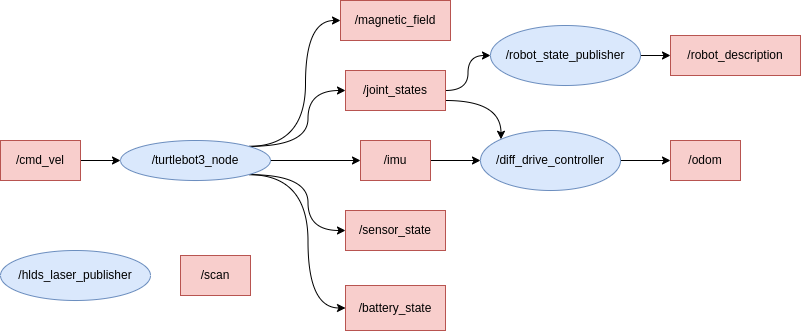
\includegraphics[width = 1\textwidth]{Figures/drawio/TB3_rqt.drawio.png}
    \caption{TurtleBot3 software map}
    \label{fig:TB3SW}
\end{figure}
\begin{figure}[H]
    \centering
    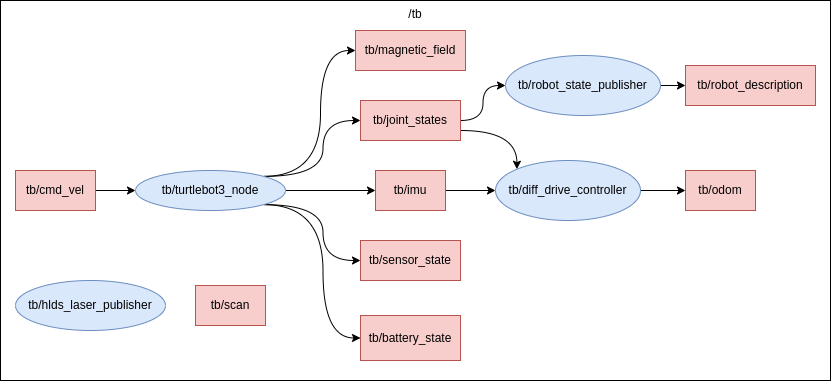
\includegraphics[width = 1\textwidth]{Figures/drawio/TB3_ns_rqt.drawio.png}
    \caption{TurtleBot3 with namespace software map}
    \label{fig:TB3nsSW}
\end{figure}

To achieve namespace like in Figure \ref{fig:TB3nsSW} $tb3\_cpp$ package was made in the $masteruia$ GitHub \cite{masteruia}. This contains three folders launch, params and src. In launch the "tb3\_launch.py" is the only one used the rest is leftovers from working. "tb3\_launch.py" is  a launch file based on using the "robot.launch.py" from "turtlebot3\_bringup" \cite{turtlebot3galactic} to launch the TB3. Here is how it works in order: 
\begin{enumerate}
\item Exporting "TURTLEBOT3\_MODEL" is required by "robot.launch.py" 
\item Opens access to LiDAR and OpenCR1.0 
\item Pushing namespace to TB3 
\item Finding and executing standard TB3 launch
\item Passing in custom parameters file for to add namespace to all the nodes 
\end{enumerate}  

The "params" folder is full of work leftovers except for "tb3\_param.yaml" witch is a copy of the standard TB3 waffle parameter file with "tb:" added in front of the nodes for namespacing.

Last folder "src" contains nodes from this project. "cmd\_vel\_subpub\_v1.py is the algorithm Time Delay \ref{Platooning_algorithm}. "feedback.py", "nav2.py", "pose\_pub\_v*.py" and "pose\_sub\_v*.py" is nodes used when attempting to use Nav2 API for a platooning algorithm \ref{Platooning_algorithm}.

%aj algorithm required or flowchart here. The implementation explained can be moved to appendix 
\section{Autonomous driving on Husky and TB3 independently}
Both robots where set up to drive autonomous and is able to do so independently. In the beginning it was thought this was necessary to archive autonomous platooning. There where two ways the robots could drive autonomous with and without a pre made map. 

Driving with simultaneous localization and mapping (SLAM) , and navigation or without a pre made map. First the base of the robot is launched, then SLAM lastly navigation. There are multiple ways of launching SLAM: 
\begin{lstlisting}[language=bash]
    ros2 launch slam_toolbox lifelong_launch.py 
    ros2 launch slam_toolbox online_async_launch.py
    ros2 launch slam_toolbox online_sync_launch.py
\end{lstlisting}
Read more about SLAM here \cite{slamtoolboxgithub}. All of the methods worked but "online\_async" was the most consistent and used. 

Here is how the Husky was launched to SLAM and navigate: 
Terminal 1: 
\begin{lstlisting}[language=bash]
    source /opt/ros/foxy/setup.bash
    source uia_husky_0776/install/local_setup.bash
    ros2 launch husky_group husky.launch.py
\end{lstlisting}
Terminal 2, note "use\_sim\_time:=false because" its not a simulation 
\begin{lstlisting}[language=bash]
    source /opt/ros/galactic/setup.bash
    ros2 launch slam_toolbox online_async_launch.py use_sim_time:=false
\end{lstlisting}
Terminal 3, note custom parameter file. 
\begin{lstlisting}[language=bash]
    source /opt/ros/galacitc/setup.bash
    ros2 launch nav2_bringup navigation_launch.py params_file:=uia_husky_0776/husky_group/params/nav2_params.yaml
\end{lstlisting}

The launch setup for the TB3 for SLAM and navigating at the same time: 
Terminal 1, note the "PushRosNamespace" where commented out in launch before this: 
\begin{lstlisting}[language=bash]
    source /opt/ros/galactic/setup.bash
    source masteruia/tb_ws/install/setup.bash
    ros2 launch tb3_cpp tb3_launch.py
\end{lstlisting}
Terminal 2, note "use\_sim\_time:=false because" its not a simulation 
\begin{lstlisting}[language=bash]
    source /opt/ros/galactic/setup.bash
    ros2 launch slam_toolbox online_async_launch.py use_sim_time:=false
\end{lstlisting}
Terminal 3, note custom parameter file. 
\begin{lstlisting}[language=bash]
    source /opt/ros/galacitc/setup.bash
    ros2 launch nav2_bringup navigation_launch.py 
\end{lstlisting}

Navigating with a pre made map uses the same setup for the robots, but SLAM is not launched and the localization\_launch.py is used inserted of navigation\_launch.py. The map is passed into localization\_launch.py as a argument. Map can be made using SLAM with navigation or telop. 

% basically you are doing (a) mimic and (b) platooning. so keep section name -algorithm and sub section / paragraph as mimic and platooning
\section{Platooning algorithm} \label{Platooning_algorithm}
%aj only write about what you have done. rest move to future work

Multiple methods of algorithm has been explored, "Mimic", "Time delay", "Nav2 API" and "AprilTags/ArUco". First two where completed and tested in real world. "Nav2 API" started on and not finished and "AprilTags/ArUco" where just researched. 

%aj algorithm required or flowchart here. The implementation explained can be moved to appendix 
\paragraph{Mimic} is the simplest form of platooning algorithm.  Where the Husky and TB3 receives the same \topic{cmd\_vel} from either teleop or Nav2 running on the husky.  This algorithm where set up and tested proving it works for a straight line. Mimic dose not work for non straight paths since the TB3 will turn at the same time as the Husky and therefor loose the path.

%%aj algorithm required or flowchart here. The implementation explained can be moved to appendix. rename platooning
% aj you are mixing method with implementation. What you describe here is implementation. need to discuss how this can be rewritten.
\paragraph{Time delay} is the same as mimic but with a time delay. The TB3 is launch with a namespace "tb". Husky receives \topic{cmd\_vel} form teleop or Nav2. A node called "cmd\_vel\_subpub\_v1.py" subscribes to \topic{cmd\_vel} and saves the data in a "delay array". The node publishes the data from the "delay array" under the \topic{/tb/cmd\_vel} topic". It is set up in the order so \topic{/tb/cmd\_vel} is one "delay array" behind \topic{cmd\_vel}. The TB3 stat one meter behind the Husky, therefor the "delay array" is initialised with a starting velocity so the TB3 and Husky has the same start position. Se flow chart \ref{fig:TimeDelayFlow} for visual explanation.

\begin{figure}[H]
    \centering
    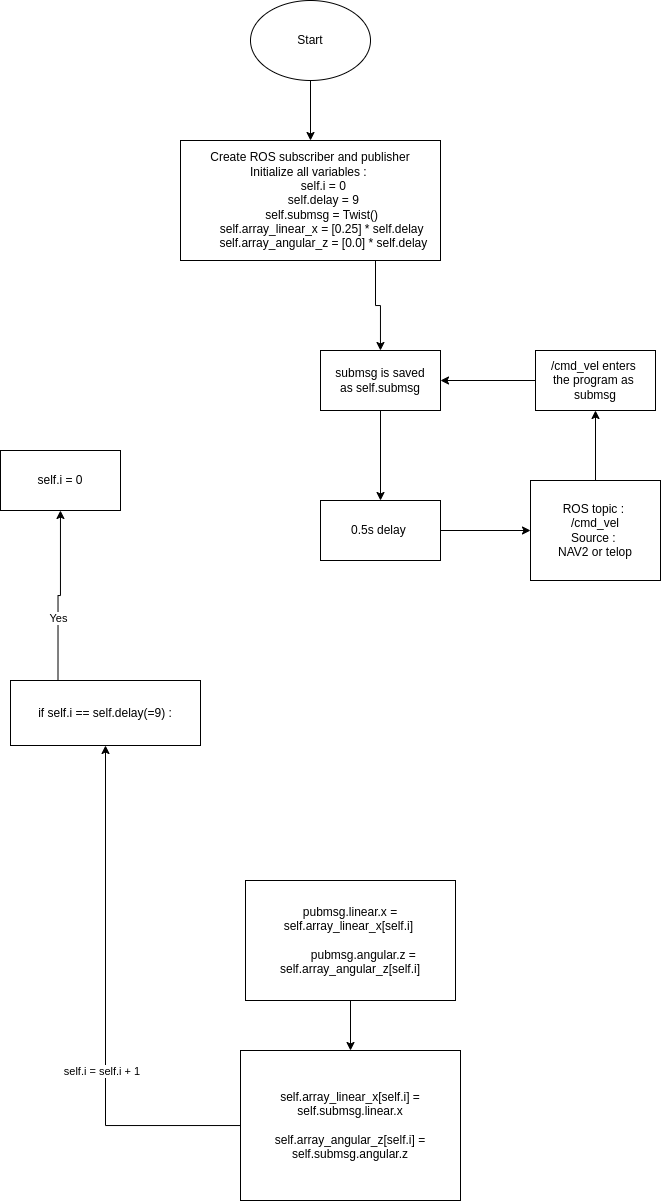
\includegraphics[width = 0.8\textwidth]{Figures/drawio/cmd_vel_subpub.png}
    \caption{Flow chart Time delay algorithm}
    \label{fig:TimeDelayFlow}
\end{figure}
%increase font size for better readiblity. explain this flow chart comprehensively
This algorithm where set up and tested and proved to be imprecise. Even though the two vehicles get the same velocity command errors accumulate over time causing the follower to drift of the path. 

%aj move to future work
\paragraph{Nav2 API} was initiated but remained unfinished due to time constraints. This method is based on the Nav2 API and the fact that the TB3 and the Husky have been setup with the ability to drive autonomously independently. For better understanding here is a list of some Nav2 API commands.

\begin{table}[H]
    \centering
    \begin{tabular}{c|c}
        Command             & Description \\ \hline
        setInitialPose()    & Setting initial pose of a robot \\
        goToPose()          & Publishes a Nav2 Goal \\
        goThroughPoses()    & Publishes a list of Nav2 Goals \\
        getPath()           & Receives the complete ongoing path \\
        changeMap()         & Changes current map to chosen one \\
        getFeedback() & Info about the robot running Nav2 like Time stamp, frame\_id and pose\\
    \end{tabular}
    \caption{Some Nav2 API commands\cite{rosnavAPI}}
    \label{tab:Nav2API}
\end{table}

The idea was both husky and TurtleBot3 run Nav2, a node receives "getFeedback()" from Husky and sends "goToPose()" x distance behind the Husky to the TB3. This task was started on but not finished here is a list with status of the milestones \ref{tab:MilestonesNav2API}.

%move to future work
\begin{table}[H]
    \centering
    \begin{tabular}{c|c}
        Task                                                        & Status   \\ \hline
        Husky driving autonomously with Nav2                        & Complete \\
        TB3 driving autonomously with Nav2                          & Complete \\
        Control Nav2 with API from python                           & Complete \\
        Husky with namespace                                        & Not complete \\
        TB3 with namespace                                          & Complete \\
        Running Nav2 on Husky with namespace                        & Not complete \\
        Running Nav2 on TB3 with namespace                          & Not complete \\
        Running Husky and TB3 on same network with independent Nav2 & Not complete\\
        Node receiving position from Husky and sending goal to TB3  & Not complete \\
    \end{tabular}
    \caption{Milestones of Nav2 API}
    \label{tab:MilestonesNav2API}
\end{table}
   


\chapter{Results on ...}

The results of this thesis is documented in this Youtube playlist \cite{youtube_playlist_results}. The playlist consist of five videos. 
Video number one called "TB w Nav2" and is showing TB3 driving autonomous using ROS2 galacitc, Nav2, SLAM Toolbox. 
The specific launch files used is : 


\chapter{Discussions}

\paragraph{Xavier}
In this project AI is not used, but can be useful for student in the future working on the same platforms. The JetPack and GPU is useless in this project. The Xavier uses ARM, and x86-64 is most used CPU architecture. Since more people are using x86-64 there are more help and software available online. 
It could be that the Xavier is amazing at AI applications and there is no product like it, i don't know. For the future i would recommend x86-64 CPU, no GPU and pure Ubuntu. A GPU dosen't hurt but not necessary unless the PC on the robot is going to run simulations or AI. Pure Ubuntu is preferable for a bigger community, faster updates and less bloat. 

\paragraph{Mimic} is not suited for autonomous platooning it works in a straigth line, if the leader turns the follower will turn at the same time and fail to follow the right path. 

\paragraph{Time delay} is not suited for autonomous platooning. In theory the the follower should copy the leader just later in time. This means if the leader stops for more that the time delay follower and leader will collide. Even though same velocity command should result in theory create the same movement for two different robots it dose not in practice. It will accumulate errors over time and drift out of the path. 


\chapter{Conclusions}

\section{Further work}
The Xaviers could be switched out with computers using x86 processor for limiting sources of error. 

\subsection{Improving platooning algorithms}
\paragraph{Time Delay} algorithm is working and can be improved with more information into the "subpub" node. The node can subscribe to odometry of Husky and TB3, and use this information to calculate the offset of where the TB3 is and where it should be. When Husky drives with Nav2 the topic \topic{/path} can be used for improving where the averness of where teh TB3 should be. Potentially LiDAR data can also be used, and the algorithm could be improved forever. Continuing improving on Time Delay feels like building a bad of Nav2. Therefor the author of this thesis believe using Nav2 API is the best way to achieve autonomous platooning with ROS2. 

\paragraph{Nav2 API} has been work on but is not finished as explained in Table \ref{tab:MilestonesNav2API}. The main challenge left is running two robots with Nav2 simultaneously on the same network. It may be that both robots need two be able to run Nav2 with namespace, but probably just one. Launching two robots may be possible with using the standard launch files from Nav2, it is also possible a custom launch file need to be build using Nav2 nodes cindo like this video \cite{MultiRobotNav2}.

\paragraph{AprilTags/ArUco} where researched but not tested. AprilTags and ArUco markers is a system where a camera can get a tf from viewing the tag seen in Figure \ref{fig:apriltags} and demonstrated in Figure \ref{fig:apriltag_principal}. When a tf between TB3 and Husky is acquired this can be used to make a platooning system or improve on an existing one. 

\begin{figure}[H]
  \centering
  \begin{minipage}[b]{0.4\textwidth}
    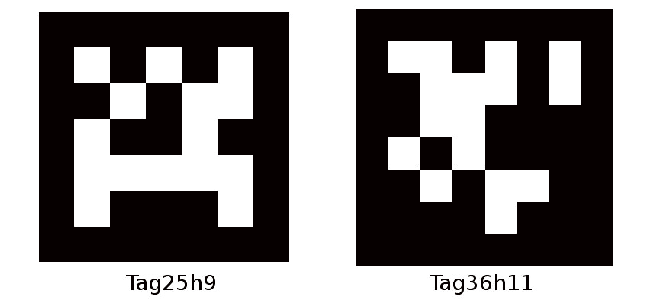
\includegraphics[width=\textwidth]{Figures/images/apriltags.png}
    \caption{Example of two AprilTags}
    \label{fig:apriltags}
  \end{minipage}
  \hfill
  \begin{minipage}[b]{0.4\textwidth}
    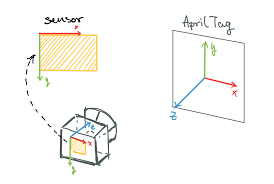
\includegraphics[width=\textwidth]{Figures/images/apriltag_prinsipal.png}
    \caption{Drawing showing the principal of AprilTags}
    \label{fig:apriltag_principal}
  \end{minipage}
\end{figure}



\appendix

\chapter{Datasheet A}


\printbibliography[
heading=bibintoc,
title={Bibliography}
]

\end{document}

